\section*{Aufgabe 2}
In der Abbildung \ref{fig:2a} sind die projezierten X-Y-Ebenen für verschiedene Startvektoren bei $r = 20$. 
Es fällt auf, dass bei dem $X$-Wert von $1$ noch ein zweites Orbital leicht auftaucht, welches sonst nicht auftritt.
In Abbildung \ref{fig:2b} sind die projezierten X-Y-Ebenen für die Lösungen mit $r = 28$ dargestellt.
Bei allen Anfangswerten sind zwei klare Orbitale zu erkennen.
\begin{figure}
    \begin{subfigure}{0.3\textwidth}
        \centering
        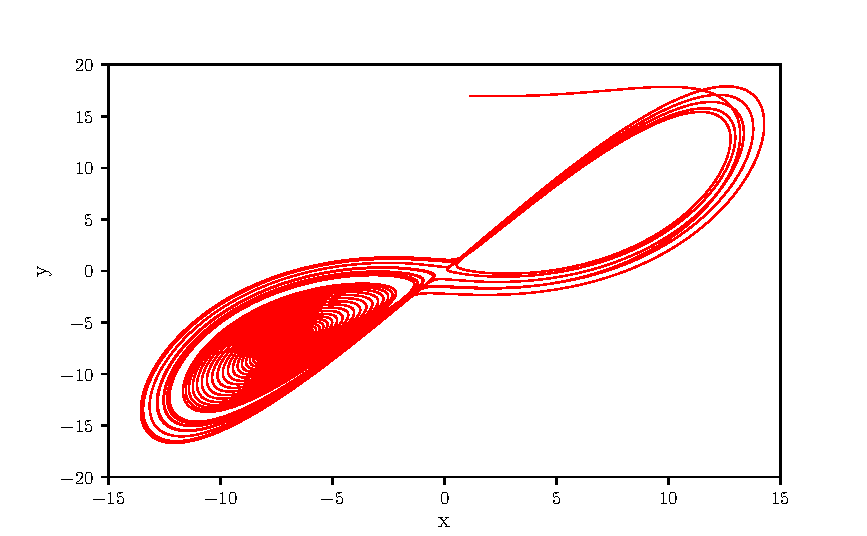
\includegraphics[height = 3.5cm]{build/pr20_1.pdf}
        \caption{$X = 1$}
    \end{subfigure}
    \hfill
    \begin{subfigure}{0.3\textwidth}
        \centering
        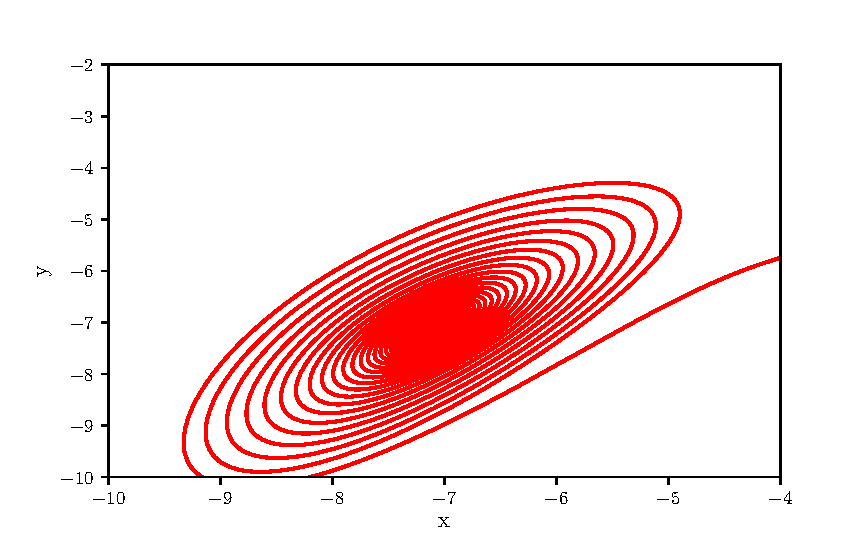
\includegraphics[height = 3.5cm]{build/pr20_23.pdf}
        \caption{$X = 23$}
    \end{subfigure}
    \hfill
    \begin{subfigure}{0.3\textwidth}
        \centering
        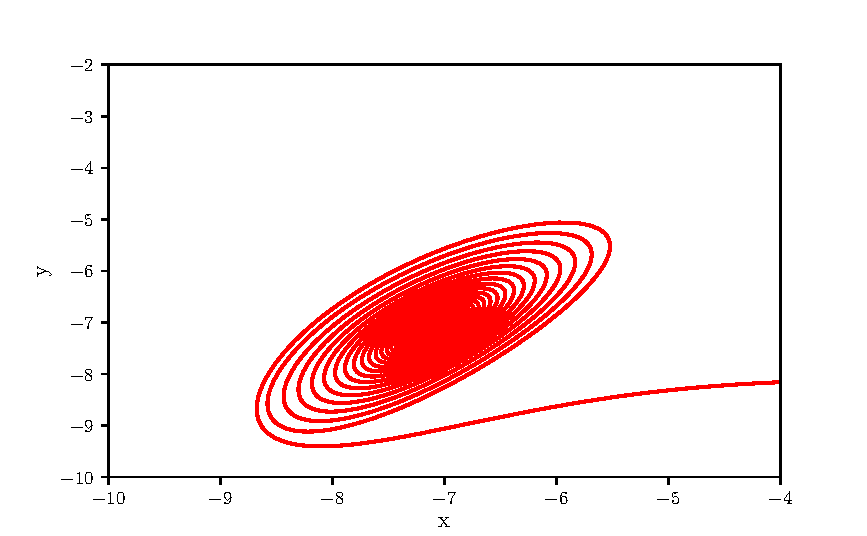
\includegraphics[height = 3.5cm]{build/pr20_32.pdf}
        \caption{$X = 32$}
    \end{subfigure}
    \caption{X-Y-Ebenen projektion bei dem Startwert $\vec{y} = (X, 17, 13)$ und mit $r = 20$.}
    \label{fig:2a}
\end{figure}
In Abbildung \ref{fig:2c} sind die 3D-plots der Poincare-Abbildung bei den verschiedenen r Werten gegeben. Die beobachtungen von der Abbildung \ref{fig:2a} und \ref{fig:2b} können hier auch wieder gezeigt werden.
\begin{figure}
    \begin{subfigure}{0.3\textwidth}
        \centering
        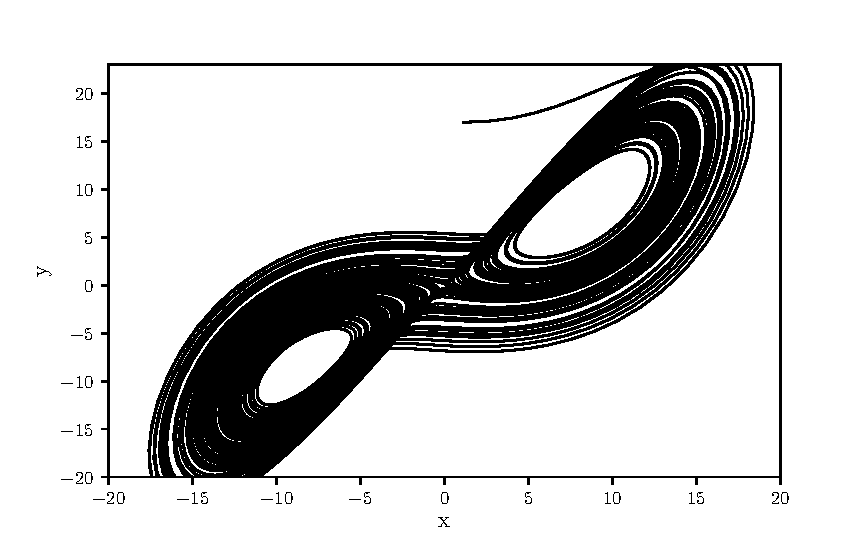
\includegraphics[height = 3.5cm]{build/pr28_1.pdf}
        \caption{$X = 1$}
    \end{subfigure}
    \hfill
    \begin{subfigure}{0.3\textwidth}
        \centering
        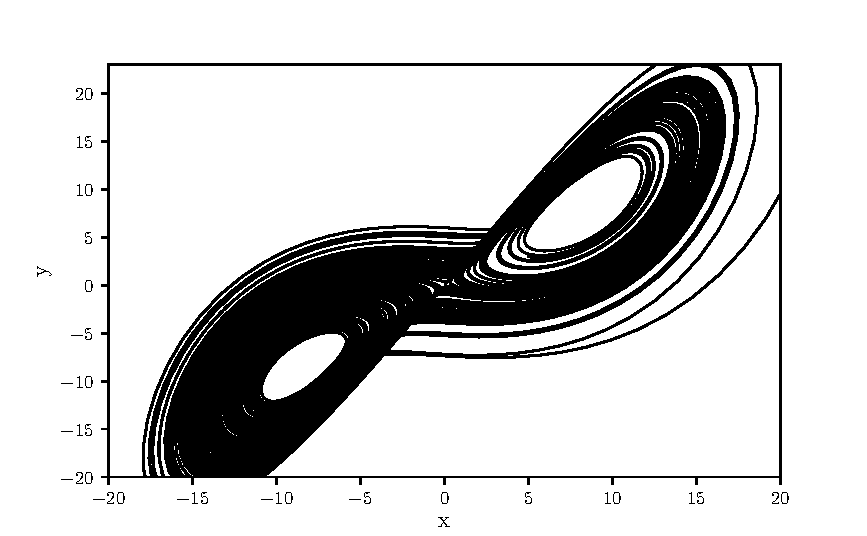
\includegraphics[height = 3.5cm]{build/pr28_23.pdf}
        \caption{$X = 23$}
    \end{subfigure}
    \hfill
    \begin{subfigure}{0.3\textwidth}
        \centering
        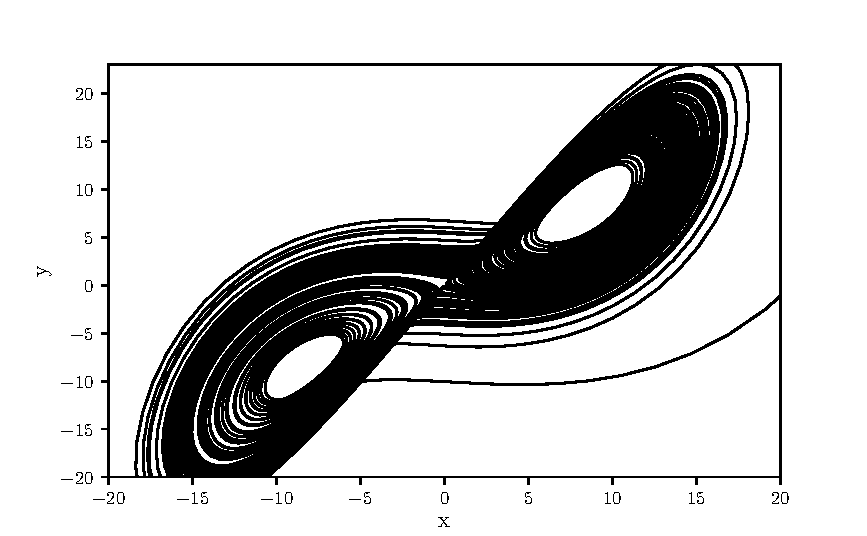
\includegraphics[height = 3.5cm]{build/pr28_32.pdf}
        \caption{$X = 32$}
    \end{subfigure}
    \caption{X-Y-Ebenen projektion bei dem Startwert $\vec{y} = (X, 17, 13)$ und mit $r = 28$.}
    \label{fig:2b}
\end{figure}

\begin{figure}
    \begin{subfigure}{0.48\textwidth}
        \centering
        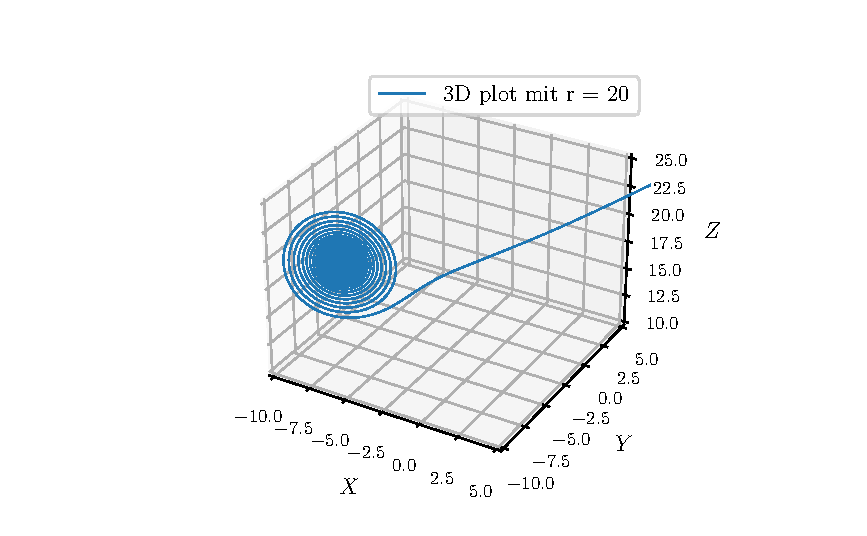
\includegraphics[height = 5.5cm]{build/pr20_3d.pdf}
        \caption{$r = 20$}
    \end{subfigure}
    \hfill
    \begin{subfigure}{0.48\textwidth}
        \centering
        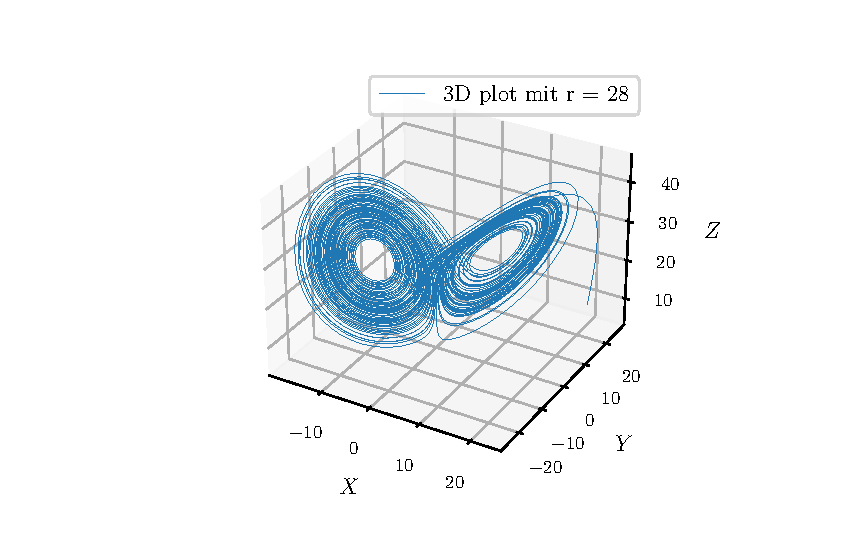
\includegraphics[height = 5.5cm]{build/pr28_3d.pdf}
        \caption{$r = 28$}
    \end{subfigure}
    \caption{3D-Plots bei dem Startwert $\vec{y} = (32, 17, 13)$ für verschiedene $r$.}
    \label{fig:2c}
\end{figure}
Die Poincare-Schnitte durch $Z = const. = 20$ bei $\dot{Z} < 0$ sind in Abbildung \ref{fig:2d} dargestellt. Dabei fällt auf, dass bei $r = 20$ nur eine gerade auftaucht, während bei 
$r = 28$ eine Ellipse auftaucht. Dies kann in Abbildung \ref{fig:2c} an den 3D-Plots gut erklärt werden. Es ist zu sehen, dass im Fall von $r = 20$ eine Schnittgerade mit
dem Orbit auftaucht. Dieser resultiert in einer geraden in der $Z = 20$-Ebene. Zusätzlich kann dem Fall $r = 28$ der zweite Orbit hinzugefügt werden. Somit kommt es zu einer zweiten Verbindungsstrecke, sodass insgesamt eine ellipse erreicht wird.
\begin{figure}
    \begin{subfigure}{0.48\textwidth}
        \centering
        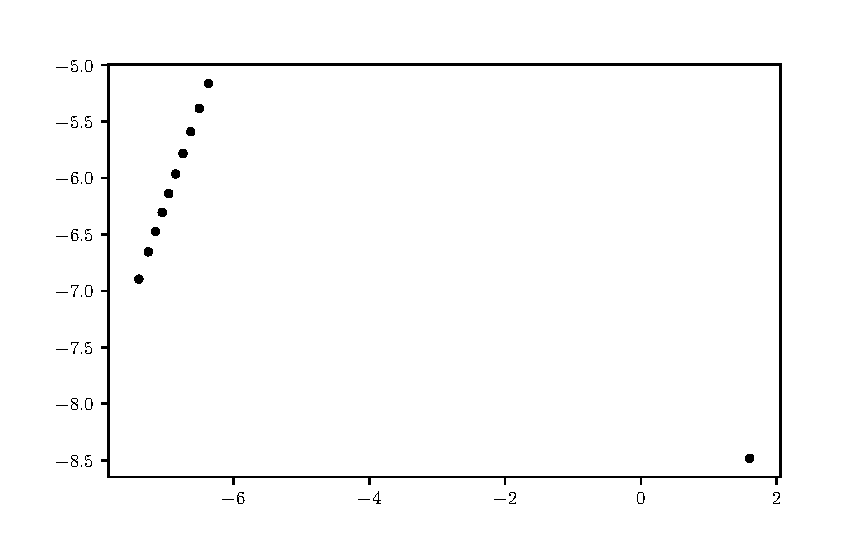
\includegraphics[height = 5cm]{build/z20_20.pdf}
        \caption{$r = 20$}
    \end{subfigure}
    \hfill
    \begin{subfigure}{0.48\textwidth}
        \centering
        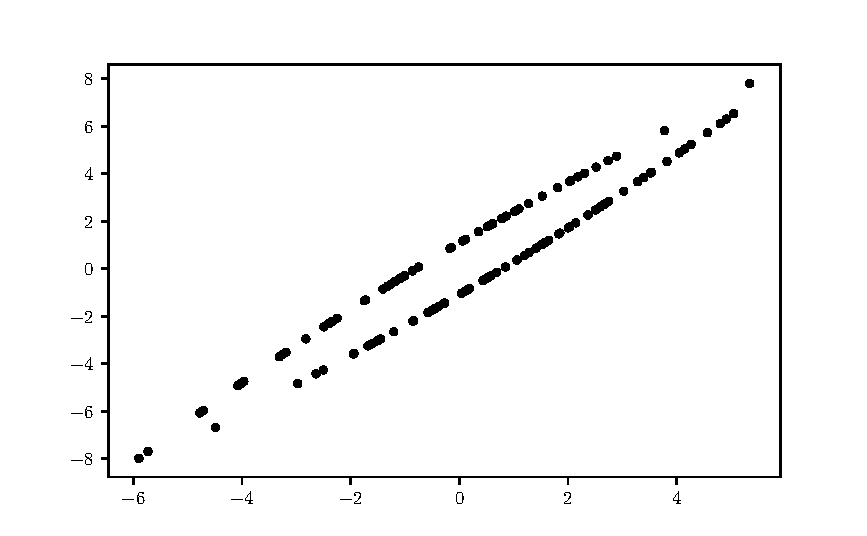
\includegraphics[height = 5cm]{build/z20_28.pdf}
        \caption{$r = 28$}
    \end{subfigure}
    \caption{Poincare-Schnitt durch $Z = 20$ bei dem Startwert $\vec{y} = (32, 17, 13)$ und mit verschiedenen $r$}
    \label{fig:2d}
\end{figure}
